\documentclass{acm_proc_article-sp}

\usepackage{graphicx}
\graphicspath{{}{./img-pdf/}}

\usepackage{color} % Allow colors to be defined
\usepackage{enumerate} % Needed for markdown enumerations to work
\usepackage{amsmath} % Equations
\usepackage{amssymb} % Equations
\usepackage[mathletters]{ucs} % Extended unicode (utf-8) support
\usepackage[utf8x]{inputenc} % Allow utf-8 characters in the tex document


\usepackage{epstopdf}


% Math Jax compatability definitions
\def\gt{>}
\def\lt{<}


\begin{document}

\newtheorem{prop}{Proposition}

\title{The Fundamental Theorem of Linear Algebra}

\numberofauthors{1}

\author{
  \alignauthor
  Alexey Grigorev\\
  Technische Universit\"at Berlin \\
  \email{grigorev@campus.tu-berlin.de}
}

\date{13 February 2015}


\maketitle


\section{Introduction}

In this report we discuss a paper ``The Fundamental Theorem of Linear Algebra" by
Gilbert Strang \cite{strang1993fundamental}. This paper is about the four
subspaces of a matrix and the actions of the matrix are illustrated visually with pictures.
The paper describes the ``Strang's diagram'', a diagram that shows
actions of \(A\), an \(m \times n\) matrix, as linear transformations
from the space \(\mathbb R^m\) to \(\mathbb R^n\). The diagram helps to
understand the fundamental concepts of Linear Algebra in terms of the
four subspaces by visually illustrating the actions of \(A\) on all
these subspaces.

The goal of this paper is to present these concepts ``in a way that
students won't forget''. The problem that the author faced is that
students have difficulties understanding Linear Algebra.
He proposes to solve this problem with the aforementioned diagrams.


There are four parts of the Fundamental Theorem of Linear Algebra: \textbf{part~1}, the dimensions of the subspaces; \textbf{part~2}, the orthogonality of the subspaces; \textbf{part~3}, the basis vectors are orthogonal; \textbf{part~4}, the matrix with respect to these bases is orthogonal. In this report, we discuss \textbf{part 1} and \textbf{part 2} only,
and describe two diagrams: the solutions to a system of linear equations
%try to be consistent with uppercase for fixed terms througout the paper
\(A \mathbf x = \mathbf b\) and the Least Squares equations. We believe
that it should give sufficient understanding to proceed with
\textbf{part 3} and \textbf{part 4}, described in the paper. Additionally,
in this report we elaborate some proofs from the paper and illustrate
the concepts with examples.


\subsection{Notation}

In this report we use the following notation: Greek lower case letter \(\alpha, \beta, \ ...\) are used for scalars, bold letters \(\mathbf b, \mathbf x, \ ...\) -- vectors, lowercase indexed letters \(x_1, x_2, \ ...\) -- components of vectors,
capital letters \(A\) -- matrices, indexed bold letters
\(\mathbf a_1, \mathbf a_2, \ ... \ , \mathbf r_1, \mathbf r_2, \ ...\)
-- columns or rows of a matrix. \(\mathbf 0\) is a vector of appropriate
dimensionality with \(0\) in each component.


\section{Fundamental subspaces and dimensionality}

A \emph{vector space} over real numbers $\mathbb R$ is a set where addition and scalar 
multiplication operations are defined in such a way that certain axioms, such as associativity,
commutativity and distributivity are satisfied \cite{strang1988book}. A \emph{subspace} is a 
subset of some vector space such that the subset is closed under addition and 
scalar multiplication, i.e.~given some subspace \(S\),
if \(\mathbf x, \mathbf y \in S\) then for any $\alpha, \beta \in \mathbb R$, \((\alpha \mathbf x + \beta \mathbf y) \in S\).

For the matrix \(A \in\mathbb R^{m \times n}\) there are four fundamental subspaces \cite{strangfour}:

\begin{itemize}
\itemsep1pt\parskip0pt\parsep0pt
\item
  \(C(A)\): the \emph{column space} of \(A\), it contains all linear combinations
  of the columns of \(A\)
\item
  \(C(A^T)\): the \emph{row space} of \(A\), it contains all linear combinations
  of the rows of \(A\) (or, columns of \(A^T\))
\item
  \(N(A)\): the \emph{nullspace} of \(A\), it contains all solutions to the system
  \(A \mathbf x = \mathbf 0\)
\item
  \(N(A^T)\): the \emph{left nullspace} of \(A\), it contains all solutions to the system
  \(A^T \mathbf y = \mathbf 0\).
\end{itemize}

All of them are subspaces because they are closed under addition and
scalar multiplication.


\subsection{Dimensionality}

These subspaces have the following dimensions: \(\operatorname{dim} C(A) = \operatorname{dim} C(A^T) = r\), where \(r\) is the rank of \(A\); \(\operatorname{dim} C(A^T) + \operatorname{dim} N(A) = n\), i.e. \(\operatorname{dim} N(A) = n - r\).
Also, \(\operatorname{dim} C(A) + \operatorname{dim} N(A^T) = m\), i.e. \(\operatorname{dim} N(A) = m - r\).


After applying Gaussian elimination for $A$ with rank $r$, in the result we get $r$ independent rows and the rest $m - r$ rows are all set to $\mathbf 0$.
Because of this, only $r$ columns have non-zero entries in the pivot position, and thus $\operatorname{dim} C(A^T) = \operatorname{dim} C(A) = r$. The rest $n-r$ columns have no pivots and correspond to free variables. The basis of \(N(A)\) is formed by \(n - r\) ``special'' solutions to \(A \mathbf x = \mathbf 0\):
we take free variables $x_{r+1}, x_{r+2}, \ ... \ , x_n$ and assign them some values, making it possible to solve the system for remaining $x_{1}, x_{2}, \ ... \ , x_r$ variables. It is possible to choose only $n-r$ linearly independent solutions, and, hence, \(\operatorname{dim} N(A) = n - r\). The same is true for $A^T$, thus, it's true for $N(A^T)$.


\subsection{Orthogonality}

Two vectors are \emph{orthogonal} if their dot product produces 0. If all vectors of one subspace are orthogonal to all vectors of another subspace, these subspaces are called \emph{orthogonal}.

\begin{prop}
The row space \(C(A^T)\) and the nullspace \(N(A)\) of \(A\) are
orthogonal. The column space \(C(A)\) and the left
nullspace \(N(A^T)\) are also orthogonal.
\end{prop}

\begin{proof}
Consider an $m \times n$ matrix $A$. Let $\mathbf r_1 , \ ... \ , \mathbf r_m$ be the rows of $A$. The row space $C(A^T)$ is formed by all linear combinations of rows, i.e. it is $\alpha_1 \mathbf r_1 + \ ... \ + \alpha_m \mathbf r_m$ for all possible choices of $\alpha_1, \ ... \ , \alpha_m$.
The nullspace $C(A)$ is formed by all the solutions $\mathbf x$ to the system $A \mathbf x = \mathbf 0$.

Let us take any vector $\mathbf r \in C(A^T)$. Because $\mathbf r \in C(A^T)$, it can be expressed as $\mathbf r = \alpha_1 \mathbf r_1 + \ ... \ + \alpha_m \mathbf r_m$. We also can take any vector $\mathbf n \in N(A)$, and because $\mathbf n \in N(A)$, we know that $A \mathbf n = \mathbf 0$. By the matrix-vector multiplication rule, the $i$th component of $A \mathbf n$ is $\mathbf r_i^T \mathbf n$ and since $A \mathbf n = \mathbf 0$, $\mathbf r_i^T \mathbf n = 0$ for all $i = 1 \ .. \ m$.

Now let us consider $\mathbf r^T \mathbf n$: $\mathbf r^T \mathbf n = \big( \alpha_1 \mathbf r_1 + \ ... \ + \alpha_m \mathbf r_m \big)^T \mathbf n = \alpha_1 \mathbf r_1^T \mathbf n  + \ ... \ + \alpha_m \mathbf r_m^T \mathbf n = \alpha_1 0 + \ ... \ + \alpha_m 0 = 0$. Thus, $\mathbf r$ and $\mathbf n$ are orthogonal, and since they are chosen arbitrarily, it holds for all $\mathbf r \in C(A^T)$ and $\mathbf n \in N(A)$.

The same is true for \(C(A)\) and \(N(A^T)\). To show this, it is enough to transpose the matrix $A$.\end{proof}

If two spaces are orthogonal and they together span the entire space,
they are called \emph{orthogonal compliments}. \(C(A^T)\) and \(N(A)\)
are orthogonal compliments as well as \(C(A)\) and \(N(A^T)\). We can illustrate this with a picture (see fig.~\ref{fig:diagram0}): the row space $C(A^T)$ and the nullspace $N(A)$ are orthogonal and meet only in the origin. They together span the space $\mathbb R^n$. $C(A)$ and $N(A^T)$ are also orthogonal and they together span $\mathbb R^m$.


\begin{figure}%[htbp]
\centering
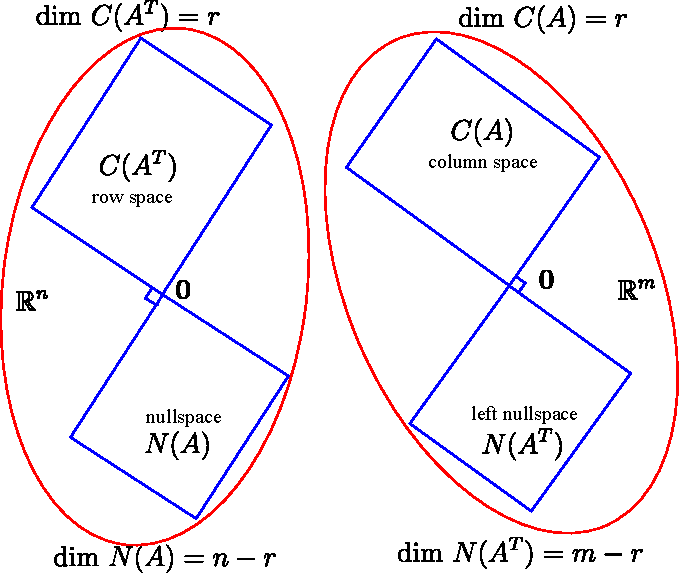
\includegraphics[width=8cm]{diagram0.pdf}
\caption{The row space $C(A^T)$ and the null space $N(A)$ are orthogonal
compliments in $\mathbb R^n$. The columns space $C(A)$ and the left nullspace $N(A^T)$ are orthogonal compliments in $\mathbb R^m$.}
\label{fig:diagram0}
\end{figure}


\newcommand\hidemath{$A \mathbf x = \mathbf b$}
\section{Solution to {\large \protect\hidemath} }
%I don't like the uppercase headings anyhow

\subsection{The row space solution}


Now we consider a system $A \mathbf x = \mathbf b$. The general solution is
\(\mathbf x = \mathbf x_p + \mathbf x_n\), where \(\mathbf x_p\) is some solution
to \(A \mathbf x = \mathbf b\), and  \(\mathbf x_n\) is the homogenous solution
to \(A \mathbf x = \mathbf 0\), because \(A \mathbf x = A (\mathbf x_p + \mathbf x_n) = A \mathbf x_p + A \mathbf x_n = \mathbf b + \mathbf 0 = \mathbf b\).


Since \(C(A^T)\) and \(N(A)\) are orthogonal compliments, they span the
entire space \(\mathbb R^n\) and every \(\mathbf x \in \mathbb R^n\) can
be expressed as \(\mathbf x = \mathbf x_r + \mathbf x_n\) such that
\(\mathbf x_r \in C(A^T)\) and \(\mathbf x_n \in N(A)\).

\begin{prop}\(\mathbf x_r\) is unique.\end{prop}

\begin{proof} Suppose there's another
solution \(\mathbf x'_r \in C(A^T)\). Since \(C(A^T)\) is a subspace,
it's close under subtraction, so
\((\mathbf x_r - \mathbf x'_r) \in C(A^T)\). Let's multiply the
difference by \(A\):
\(A(\mathbf x_r - \mathbf x'_r) = A \mathbf x_r - A \mathbf x'_r = \mathbf b - \mathbf b = \mathbf 0\).
So \((\mathbf x_r - \mathbf x'_r) \in N(A)\) and
\((\mathbf x_r - \mathbf x'_r) \in C(A^T)\). Since \(C(A^T)\) and
\(N(A)\) are orthogonal compliments, the only place where they meet is
in \(\mathbf 0\), so \(\mathbf x_r - \mathbf x'_r = \mathbf 0\) or
\(\mathbf x_r = \mathbf x'_r\). In other words, \(\mathbf x_r\) is
indeed unique.
\end{proof}


As we mentioned earlier, there are many possible choices of \(\mathbf x_p\).
Among all these choices of \(\mathbf x_p\) there's once special choice
\(\mathbf x_r\) -- the \emph{row space solution} to the system. It's
special because it belongs to the row space, and it's unique. So any
solution to \(A \mathbf x = \mathbf b\) can be written as a combination
\(\mathbf x = \mathbf x_r + \mathbf x_n\).


\subsection{Existence}

A solution to \(A \mathbf x = \mathbf b\) exists only if
\(\mathbf b \in C(A)\), i.e.~when \(\mathbf b\) is a linear combination
of columns of \(A\).

Let \(\mathbf a_i\) be the columns of \(A\), i.e. \(A = \left[ \mathop{\mathbf a_1}\limits_|^| \, \mathop{\mathbf a_2}\limits_|^| \ \cdots \  \mathop{\mathbf a_n}\limits_|^| \right]\).  Then for the solution to exist, there must exist \((x_1 , \ ... \ , x_n)\) s.t. \(x_1 \mathbf a_1 + x_2 \mathbf a_2 + \ ... \ + x_n \mathbf a_n = \mathbf b\). If these \((x_1, \ ... \ , x_n)\) exist, they form a solution \(\mathbf x = \begin{bmatrix} x_1 \\ \vdots \\ x_n \end{bmatrix}\).  Note that   \(x_1 \mathbf a_1 + x_2 \mathbf a_2 + \ ... \ + x_n \mathbf a_n = \mathbf b\) is the same as writing \(A \mathbf x = \mathbf b\).


\begin{figure}%[htbp]
\centering
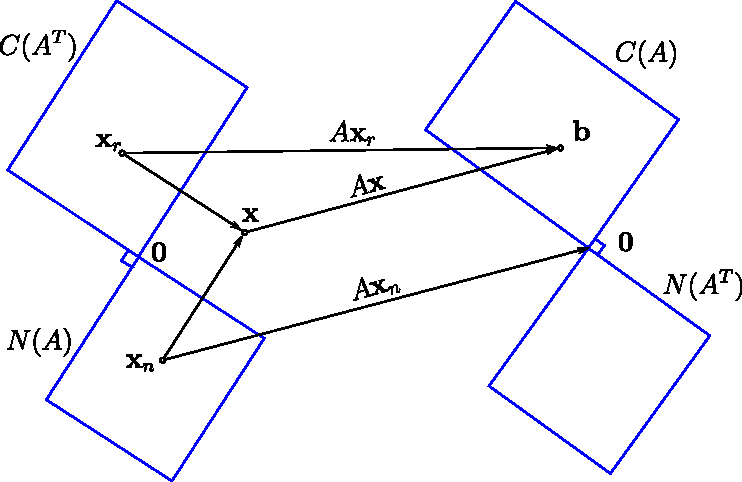
\includegraphics[width=8.5cm]{diagram1.pdf}
\caption{The general solution $\mathbf x$ to the system $A \mathbf x = \mathbf b$ consists of two components $\mathbf x_r \in C(A^T)$ and $\mathbf x_n \in N(A)$. The solution to the system exists because $\mathbf b \in C(A)$.}
\label{fig:diagram1}
\end{figure}


We can illustrate this with a diagram (see fig.~\ref{fig:diagram1}):
$\mathbf b \in C(A)$, so there is a solution $\mathbf x$ to the system.
The solution $\mathbf x$ can be expressed as $\mathbf x_r + \mathbf x_n$ s.t.
$\mathbf x_r \in C(A^T)$ and $\mathbf x_n \in N(A)$; both $A \mathbf x_r = \mathbf b$ and
$A \mathbf x = \mathbf b$, and it is shown with arrows to $\mathbf b$.


\subsection{Example}

Consider a system with
\(A = \begin{bmatrix} 1 & 1 & 1 \\ 1 & 2 & 3 \\ 2 & 3 & 4 \end{bmatrix}\)
and \(\mathbf b = \begin{bmatrix} 0 \\ 1 \\ 1 \end{bmatrix}\).


Let us first find the column space \(C(A)\): it is formed by linear combinations \(\alpha_1 \begin{bmatrix} 1 \\ 1 \\ 2 \end{bmatrix} + \alpha_2 \begin{bmatrix} 1 \\ 2 \\ 3 \end{bmatrix} + \alpha_3 \begin{bmatrix} 1 \\ 3 \\ 4 \end{bmatrix}\) for all possible choices of \((\alpha_1, \alpha_2, \alpha_3)\).

To check if the system \(A \mathbf x = \mathbf b\) has a solution, we need to show that \(\mathbf b \in C(A)\). In other words, we need to show that it is possible to find such \(\mathbf x = \begin{bmatrix} x_1 \\ x_2 \\ x_3 \end{bmatrix}\) that \(x_1 \begin{bmatrix} 1 \\ 1 \\ 2 \end{bmatrix} + x_2 \begin{bmatrix} 1 \\ 2 \\ 3 \end{bmatrix} + x_3 \begin{bmatrix} 1 \\ 3 \\ 4 \end{bmatrix} = \begin{bmatrix} 0 \\ 1 \\ 1 \end{bmatrix}\).
In this example $x_1 = -1, x_2 = 1$ and $x_3 = 0$:
\(-1 \begin{bmatrix} 1 \\ 1 \\ 2 \end{bmatrix} + 1 \begin{bmatrix} 1 \\ 2 \\ 3 \end{bmatrix} + 0 \begin{bmatrix} 1 \\ 3 \\ 4 \end{bmatrix} = \begin{bmatrix} 0 \\ 1 \\ 1 \end{bmatrix}\).
Note that here we not only established that \(\mathbf b \in C(A)\), but also found a solution
\(\mathbf x_p = \begin{bmatrix} x_1 \\ x_2 \\ x_3 \end{bmatrix} = \begin{bmatrix} 1 \\ -1 \\ 0 \end{bmatrix}\). This solution is not necessarily the row space solution, i.e.~it may not belong to the row space \(C(A^T)\).

The nullspace \(N(A)\) contains all the solutions to
\(A \mathbf x = \mathbf 0\). To find them, we use Gaussian Elimination and transform \(A\) to the Row-Reduced Echelon Form:
\(\begin{bmatrix} 1 & 1 & 1 \\ 1 & 2 & 3 \\ 2 & 3 & 4 \end{bmatrix} \to \begin{bmatrix} 1 & 0 & -1 \\ 0 & 1 & 2 \\ 0 & 0 & 0 \end{bmatrix}\).
There are two pivot variables \(x_1\) and \(x_2\): they have \(1\) at the
pivot position, and there is one free variable \(x_3\) that doesn't have a pivot: it has
\(0\) on this position.
The free variable can take any value, for example, we can assign \(x_3 = 1\).
Then we have \(x_n = \begin{bmatrix} x_1 \\ x_2 \\ 1 \end{bmatrix}\),
we solve the system and obtain \(x_1 = 1, x_2 = -2\), so the solution is \(x_n = \begin{bmatrix} 1 \\ -2 \\ 1 \end{bmatrix}\).
There is nothing special about the choice \(x_3 = 1\), so instead we
can choose \(x_3 = \alpha\), and obtain \(x_n = \begin{bmatrix} \alpha \\ -2 \alpha \\ \alpha
\end{bmatrix} = \alpha \begin{bmatrix} 1 \\ -2 \\ 1 \end{bmatrix}\). All possible choices of $\alpha$ form the nullspace \(N(A)\).


The complete solution $\mathbf x$ is a sum of some solution and the homogenous solutions:
\(\mathbf x = \mathbf x_p + \mathbf x_n = \begin{bmatrix} 0 \\ 1 \\ 1 \end{bmatrix} + \alpha
\begin{bmatrix} 1 \\ -2 \\ 1 \end{bmatrix}\). Note that the set of all solutions $\mathbf x$ is
just a shifted nullspace $N(A)$ (see fig.~\ref{fig:row-space-x-special}).

Because the rank of $A$ is two, the row space $C(A^T)$ contains only two linearly independent
vectors, so it is a plane in \(\mathbb R^3\) formed by two rows $\mathbf r_1$ and $\mathbf r_2$. The row space solution $\mathbf x_r$ also belongs to $C(A^T)$, but the solution $\mathbf x_p = \begin{bmatrix} 1 \\ -1 \\ 0 \end{bmatrix}$ does not (see fig.~\ref{fig:row-space-x-special}). If we want to find \(\mathbf x_r\), at first we need to recognize that it's a projection of \(\mathbf x_p\) onto \(C(A^T)\). We will see how to find
this projection in the next section.

\begin{figure}%[htbp]
\centering
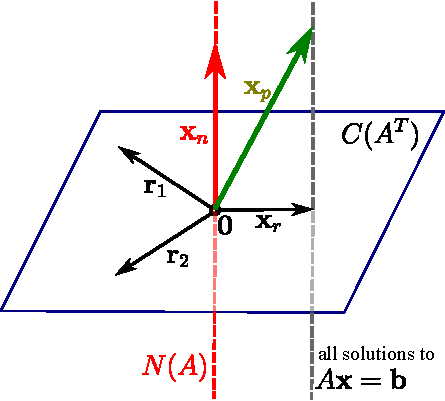
\includegraphics[width=4cm]{row-space-x-special3.pdf}
\caption{The basis of $C(A^T)$ is two rows of $A$, $N(A)$ is orthogonal to $C(A^T)$, and the set of all solutions $\mathbf x$ is just shifted $N(A)$. The row space solution $\mathbf x_r$ belongs to $C(A^T)$ and it's a solution to the system.}
\label{fig:row-space-x-special}
\end{figure}



\section{The Least Squares}

Sometimes there is no solution to the system $A \mathbf x = \mathbf b$.

For example, consider a system \(\begin{bmatrix} 1 & 1 \\ 1 & 2 \\ 1 & 3 \end{bmatrix} \begin{bmatrix} x_1 \\ x_2 \end{bmatrix} = \begin{bmatrix} 1 \\ 0 \\ 0 \end{bmatrix}\). The column space of \(A\) is
\(C(A) = \alpha_1 \begin{bmatrix} 1 \\ 1 \\ 1 \end{bmatrix} + \alpha_2 \begin{bmatrix} 1 \\ 2 \\ 3 \end{bmatrix}\). But for this $\mathbf b$ it is not possible to find such $\alpha_1, \alpha_2$ that would produce $\mathbf b$: it is not a combination of columns of \(A\), thus
\(\mathbf b \not \in C(A)\) and therefore there is no solution to \(A \mathbf x = \mathbf b\). What if we still need to find some solution to this system, not necessarily exact, but as good as possible?


\subsection{Projection on column space}

So the goal is to find some approximation \(\hat {\mathbf x}\) such that \(A \hat {\mathbf x} \in C(A)\). To do it, we need $\mathbf p$ to be as close as possible to the original \(\mathbf b\).
Such $\mathbf p$ is called a \emph{projection} of $\mathbf b$ onto $C(A)$.
Let \(\mathbf e = \mathbf b - \mathbf p\) be the \emph{projection error}.
The projection error need to be as small as possible (see fig.~\ref{fig:least-squares-proj}).


\begin{figure}
\centering
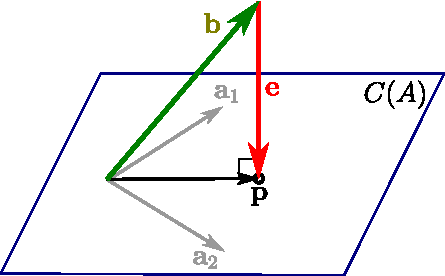
\includegraphics[width=4cm]{least-squares-proj.pdf}
\caption{$\mathbf b \not \in C(A)$, so there's no solution to $A \mathbf x = b$. $\mathbf p \in C(A)$ is a projection of $\mathbf b$ onto $C(A)$, so there exists a solution to $A \hat {\mathbf x} = \mathbf p$.}
\label{fig:least-squares-proj}
\end{figure}

\begin{prop}
The projection error \(\mathbf e\) is minimal, when it's perpendicular to \(C(A)\).
\end{prop}

\begin{proof}
Let \(\mathbf e = \mathbf b - \mathbf p\) be perpendicular to $C(A)$ and consider another vector \(\mathbf p' \in C(A)\), \(\mathbf p' \ne \mathbf p\) such that
\(\mathbf e' = \mathbf b - \mathbf p'\) is not perpendicular to
\(C(A)\). Then, by the Pythagoras theorem, \(\| \mathbf e' \|^2 = \| \mathbf e \|^2 + \| \mathbf p - \mathbf p' \|^2 > \| \mathbf e \|^2\), so \(\| \mathbf e' \| > \| \mathbf e \|\) for any
\(\mathbf e' \ne \mathbf e\) (see fig.~\ref{fig:smallest-error}). Thus, \(\mathbf e\) is smallest when it is perpendicular to $C(A)$.
\end{proof}


\begin{figure}%[htbp]
\centering
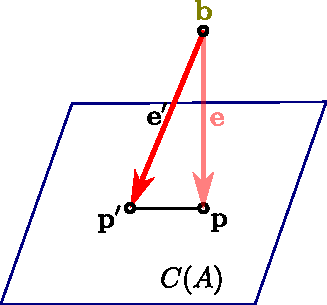
\includegraphics[width=3cm]{smallest-error.pdf}
\caption{The projection error \(\mathbf e\) is smallest when it's perpendicular to \(C(A)\).}
\label{fig:smallest-error}
\end{figure}

We need to find such \(\hat {\mathbf x}\) that \(\mathbf e\) is smallest. $\mathbf e$ is smallest when it's orthogonal to \(C(A)\), i.e. to all vectors on \(C(A)\): \(\mathbf a_1^T \mathbf e = \mathbf 0\) and \(\mathbf a_2^T \mathbf e = \mathbf 0\).  We can write the same as \(A^T \mathbf e = \mathbf 0\). Since \(\mathbf e = \mathbf b - \mathbf p = \mathbf b - A \hat {\mathbf x}\) and \(A^T \mathbf e = \mathbf 0\), we have \(A^T (\mathbf b - A \hat {\mathbf x}) = \mathbf 0\) or \(A^T A \hat {\mathbf x} = A^T \mathbf b\). This is called the \emph{Normal Equation} and it minimizes the error \(\mathbf e\). The \emph{Least Squares solution} is \(\hat {\mathbf x} = (A^T A)^{-1} A^T \mathbf b\).

There is another way to arrive at the same solution using calculus. Suppose we want to minimize the sum of squared errors \(\| \mathbf e \|^2\). So the goal is to find such \(\mathbf x\)
that minimizes \(\| \mathbf e \|^2 = \| \mathbf b - A \mathbf x \|^2\). First, expand it as
\(\| \mathbf b - A \mathbf x \|^2 = ( \mathbf b - A \mathbf x )^T ( \mathbf b - A \mathbf x ) = \mathbf b^T \mathbf b - 2 \mathbf x^T A^T \mathbf b + \mathbf x^T A^T A \mathbf x\).
Now by taking the derivative w.r.t. \(\mathbf x\) and we obtain
\(- 2 A^T \mathbf b + 2 A^T A \hat {\mathbf x} = \mathbf 0\) or \(A^T A \hat {\mathbf x} = A^T \mathbf b\). We come to the same conclusion, and because we minimized the squared error, this technique is called ``Least Squares''.


There is one additional condition: \(A^T A\) is invertible only if \(A\) has
independent columns. \(A\) has independent columns when \(N(A) = \{ \ \mathbf 0 \ \}\),
so it is enough to show that \(A^T A\) and \(A\) have the same nullspaces.

\begin{prop}\(N(A) \equiv N(A^T A)\)\end{prop}

\begin{proof}In this proof, we show that both \(N(A^T A) \subseteq N(A)\) and \(N(A) \subseteq N(A^T A)\) hold at the same time, and hence \(N(A) \equiv N(A^T A)\).

First, we prove that if \(A^T A \mathbf x = \mathbf 0\) then \(A \mathbf x = \mathbf 0\),
i.e. \(N(A^T A) \subseteq N(A)\). Suppose \(\mathbf x\) is a solution to
\(A^T A \mathbf x = \mathbf 0\). By multiplying it by \(\mathbf x^T\) we get
\(\mathbf x^T A^T A \mathbf x = \mathbf 0\). A dot product of vector with itself is a squared
$L_2$ norm, so we have \(\|A \mathbf x \|^2 = \mathbf 0\). A vector can have length $0$ only if
it is a zero vector, so \(A \mathbf x = \mathbf 0\). Thus, $\mathbf x$ is a solution to
\(A \mathbf x = \mathbf 0\) as well.

Next, we show that if \(A \mathbf x = \mathbf 0\) then
\(A^T A \mathbf x = \mathbf 0\), i.e. \(N(A) \subseteq N(A^T A)\).
If \(\mathbf x\) is a solution to \(A \mathbf x = \mathbf 0\), then by multiplying it by
\(A^T\) on the left we get \(A^T A \mathbf x = \mathbf 0\).

Since \(N(A^T A) \subseteq N(A)\) and \(N(A) \subseteq N(A^T A)\),
we conclude that \(N(A) \equiv N(A^T A)\).\end{proof}


\begin{figure}%[htbp]
\centering
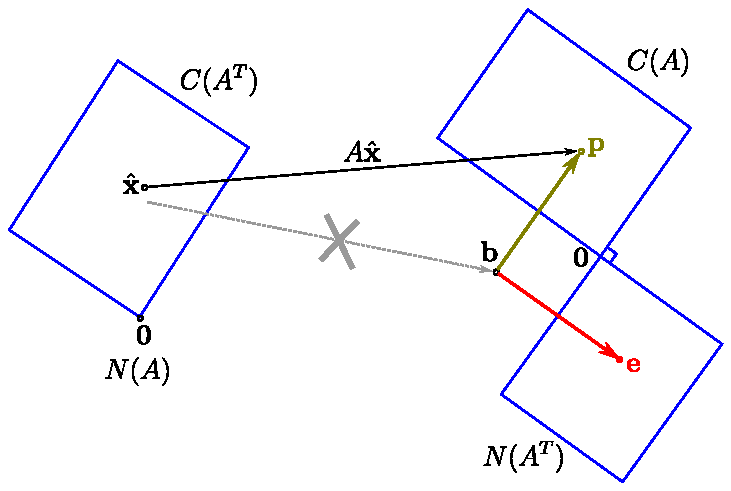
\includegraphics[width=8.5cm]{diagram2-least-squares.pdf}
\caption{There is no solution to $A \mathbf x = \mathbf b$ because $\mathbf b \not \in C(A)$, but the projection $\mathbf p \in C(A)$ and there's a solution to $A \hat {\mathbf x} = \mathbf p$. The projection error $\mathbf e \in N(A^T)$ and $N(A)$ is empty: it contains only $\mathbf 0$.}
\label{lab:diagram2-least-squares}
\end{figure}


This technique can be illustrated by the diagram as well (see fig.~\ref{lab:diagram2-least-squares}): \(\mathbf b\) is not in \(C(A)\), so we can't solve the system, but we can project \(\mathbf b\) onto \(C(A)\) to get \(\mathbf p\) and then
solve \(A \hat {\mathbf x} = \mathbf p\) . Note that
\(\mathbf b = \mathbf p +\mathbf e\), and \(\mathbf e \in N(A^T)\). This is because
to obtain the Normal Equation we solve \(A^T \mathbf e = \mathbf 0\), and the left nullspace
\(N(A^T)\) contains all the solutions to \(A^T \mathbf y = \mathbf 0\).


\subsection{Example}

Consider a system with \(A = \begin{bmatrix} 1 & 1 \\ 1 & 2 \\ 1 & 3 \end{bmatrix}\),
and \(\mathbf b =\begin{bmatrix} 1 \\ 0 \\ 0 \end{bmatrix}\). To solve \(A^T A \hat {\mathbf x} = A^T \mathbf b\), we first calculate \(A^T A = \begin{bmatrix} 1 & 1 & 1 \\ 1 & 2 & 3 \end{bmatrix}
\begin{bmatrix} 1 & 1 \\ 1 & 2 \\ 1 & 3 \end{bmatrix} = \begin{bmatrix} 3 & 6 \\ 6 & 14
\end{bmatrix}\).
Then, we calculate \(A^T \mathbf b = \begin{bmatrix} 1 & 1 & 1 \\ 1 & 2 & 3 \end{bmatrix}
\begin{bmatrix} 1 \\ 0 \\ 0 \end{bmatrix} = \begin{bmatrix} 1 \\ 1 \end{bmatrix}\).
Now we solve the system \(\begin{bmatrix} 3 & 6 \\ 6 & 14 \end{bmatrix} \hat {\mathbf x} = \begin{bmatrix} 1 \\ 1 \end{bmatrix}\) and the solution is
\(\hat {\mathbf x} = \begin{bmatrix} 4/3 \\ -1/2 \end{bmatrix}\).

What if \(A\) did not have independent columns? Suppose \(A = \begin{bmatrix} 1 & 2 \\ 1 & 2 \\ 1 & 2 \end{bmatrix}\). Then \(A^T A = \begin{bmatrix} 3 & 6 \\ 6 & 12 \end{bmatrix}\). This
matrix is singular, i.e.~it doesn't have the inverse, and thus we cannot
solve the system \(A^T A \hat {\mathbf x} = A^T \mathbf b\).


\subsection{Application: OLS Regression}

The Least Squares method is commonly used in Statistics and Machine Learning to find
a best fit line for a given data data set. This method is called
\emph{OLS Regression} (\emph{Ordinary Least Squares Linear Regression})
or just \emph{Linear Regression}.

\textbf{Linear Regression problem}:

Given a dataset \(\mathcal D = \{ \ (\mathbf x_i, y_i) \ \}\) of \(n\) pairs \((\mathbf x_i, y_i)\) where \(\mathbf x_i \in \mathbb R^d\) and
\(y_i \in \mathbb R\) we train a model that can predict \(y\) for new unseen data points \(\mathbf x\) as good as possible. To do this, we fit a line \(y = w_0 + w_1 x_1 + w_2 x_2 + \ ... \ + w_d x_d\).
This is the \emph{best fit line}, \(w_0\) is the \emph{intercept} coefficient, and
\(w_1, \ ... \ , w_n\) are the \emph{slope} coefficients. Let \(x_0 = 1\), so we can write \(y = w_0 x_0 + w_1 x_1 + w_2 x_2 + \ ... \ + w_d x_d = \mathbf w^T \mathbf x\).
Let \(\mathbf X = \begin{bmatrix} - \ \mathbf x_1 \ - \\ - \ \mathbf x_2 \ - \\ \vdots \\ - \ \mathbf x_n \ - \end{bmatrix}\). This \(\mathbf X\) is called the \emph{data matrix} and its rows are formed by \(\mathbf x_i\). \(\mathbf X\) is a \(n \times (d + 1)\) matrix. Also let \(\mathbf w = \begin{bmatrix} w_0 \\ w_1 \\ \vdots \\ w_d \end{bmatrix} \in \mathbb R^{d+1}\) and
\(\mathbf y = \begin{bmatrix} y_1 \\ y_2 \\ \vdots \\ y_n \end{bmatrix} \in \mathbb R^n\).

We need to solve the system \(\mathbf X \mathbf w = \mathbf y\), but usually there is no solution, so we use the Normal Equation, and the Least Squares solution to this problem is given by \(\hat {\mathbf w} = (\mathbf X^T \mathbf X)^{-1} \mathbf X^T \mathbf y\).


\textbf{Example}. Consider a dataset \(\mathcal D = \{(1,1), (2,0), (3,0) \}\). We add \(w_0 = 1\) to each observation and have \(\mathbf x_1 = \begin{bmatrix} 1 \\ 1 \end{bmatrix}, \mathbf x_2 = \begin{bmatrix} 1 \\ 2 \end{bmatrix}, \mathbf x_3 = \begin{bmatrix} 1 \\ 3 \end{bmatrix}\).
Let \(\mathbf X = \begin{bmatrix} - \ \mathbf x_1 \ - \\ - \ \mathbf x_2 \ - \\ - \ \mathbf x_3 \ - \end{bmatrix} = \begin{bmatrix} 1 & 1 \\ 1 & 2 \\ 1 & 3 \end{bmatrix}\)
and
\(\mathbf y = \begin{bmatrix} y_1 \\ y_2 \\ y_3 \end{bmatrix} = \begin{bmatrix} 1 \\ 0 \\ 0 \end{bmatrix}\). Then \(\hat {\mathbf w} = (\mathbf X^T \mathbf X)^{-1} \mathbf X^T \mathbf y = \begin{bmatrix} 4/3 \\ -1/2 \end{bmatrix}\) (see fig.~\ref{fig:ols}).


\begin{figure}%[htbp]
\centering
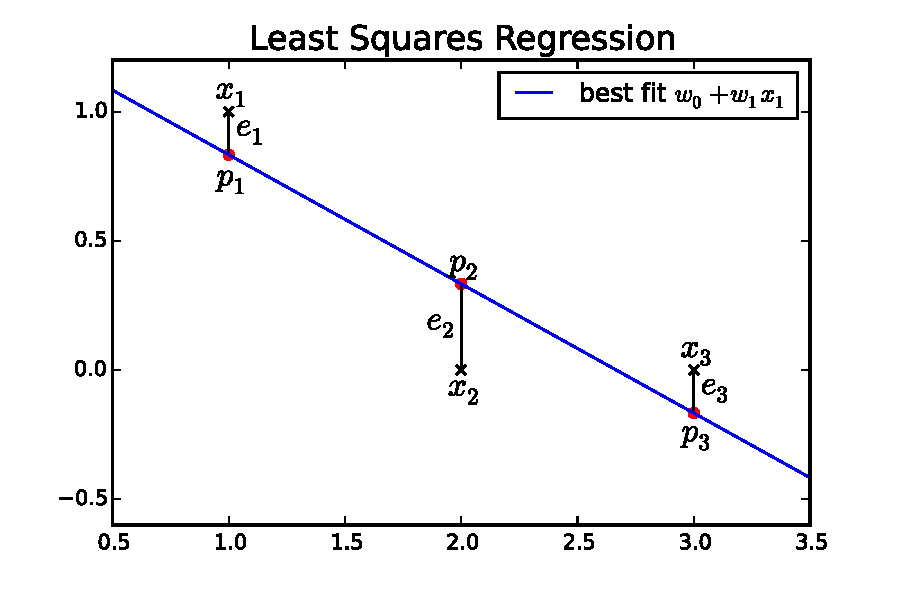
\includegraphics[width=9cm]{ols.pdf}
\caption{The best fit line with $w_0 = 4/3$ and $w_1 = -1/2$. $x_1, x_2, x_3$ are the data points, $p_1, p_2, p_3$ are OLS predictions, and $e_1, e_2, e_3$ are prediction errors.}
\label{fig:ols}
\end{figure}



\section{Conclusion}

The paper presents the ``Strang's diagram'' for helping students to understand Linear Algebra better. The purpose of this paper is educational, there is no novelty (the pictures had been presented earlier in the author's textbook \cite{strang1988book}) and no research. Also, the claim that the pictures illustrate actions of the matrix ``in a way they [the students] won't forget'' is not supported by any statistical evaluation.
And finally, the reader should already be familiar with concepts of Linear Algebra to understand the paper, and there are no supporting examples.

However, the presented diagram is indeed an effective tool for illustrating the four fundamental
subspaces and their relation to the important concepts like orthogonality, solution existence,
projections, all in one place in a concise form.
It also helps to think of many Linear Algebra problems, such as solving the system $A \mathbf x = \mathbf b$ or finding the Least Squares solution, in terms of the subspaces and it is
very beneficial for understanding these problems.

Lastly, the paper summarizes the author's textbook \cite{strang1988book} and therefore reading
the paper is a good way of refreshing the key concepts of Linear Algebra.


\bibliographystyle{abbrv}
\bibliography{imsem}


\balancecolumns
\end{document}
